\chapter{Especificación}
\label{cap:especificacion}
En este capítulo se detallan los requisitos del proyecto y se describen los casos de uso de la aplicación interactiva.

\bigskip
El objetivo del proyecto es construir un entorno interactivo que permita jugar y  comparar las diferentes estrategias de juego en IA.
% poner en introducción (objetivos).
%Este entorno interactivo esta basado en una aplicación Java.

\section{Requisitos}
\label{sec:requisitos}
El proyecto puede dividirse en dos partes bien diferenciadas: por un lado el módulo de razonamiento de los agentes junto con los juegos; por otro lado la aplicación interactiva, es decir, la interfaz gráfica de usuario.
Teniendo esto en cuenta se pueden extraer los requisitos de ambas partes de forma separada.

\bigskip
A continuación se presentan primero las características del módulo de razonamiento y después la aplicación gráfica de usuario.

\subsection{Módulo de razonamiento}
\label{ssec:modulo_razonamiento}
El proyecto incluye un módulo de razonamiento para los agentes jugadores y los juegos.

Los algoritmos de decisión deben ser independientes de los propios juegos, es decir, en cada juego debe poder usarse todos los algoritmos disponibles.
Esto es complicado pues hay estrategias que necesitan de información concreta sobre el estado de los juegos para evaluar las posiciones.
Para solucionarlo se separarán también los evaluadores heurísticos de los algoritmos que los usan, independizando totalmente los algoritmos de los juegos.

Los juegos tienen las siguientes características: juegos de dos jugadores, por turnos, de suma cero, de información perfecta y deterministas.
El módulo se completará con la implementación de dos juegos:
\begin{itemize}
\renewcommand{\labelitemi}{$\bullet$}
	\item El juego del Conecta-4; considerando una versión generalizada del mismo con un tamaño de tablero \textit{nxm} y una longitud ganadora de \textit{k} fichas.
	Las pruebas se realizarán sobre tableros de dimensiones 4x4 y 6x7 con longitudes ganadores de tres y cuatro fichas respectivamente.
	\item El juego del Go; considerando una versión generalizada del mismo con un tamaño de tablero \textit{nxn}.
	Las pruebas se realizarán sobre un tablero de dimensiones 9x9.
\end{itemize}
Ambos juegos deben ser representados mediante un espacio de estados que entiendan todos los algoritmos.

Por otro lado, los algoritmos o estrategias deben ajustarse a un espacio de estados genérico, independiente del juego.
Se tratará de versiones generales de los algoritmos, de forma que resulten sencillas de entender.
Los jugadores que se desarrollarán son los presentados a continuación cuyas respectivas estrategias han sido estudiadas en el capítulo~\ref{cap:estrategias}:
\begin{itemize}
\renewcommand{\labelitemi}{$\bullet$}
	\item Un jugador humano, que será el único jugador totalmente dependiente del juego, pues es necesario que pida el movimiento a realizar al usuario mediante un dispositivo de entrada como el teclado o el ratón.
	\item Un jugador con estrategia aleatoria.
	\item Un jugador con evaluador heurístico.
	\item Un jugador con estrategia minimax y una profundidad máxima de búsqueda fijada.
	\item Un jugador con estrategia minimax y un tiempo limitado para realizar la búsqueda.
	\item Un jugador con poda alfa-beta y una profundidad máxima de búsqueda.
	\item Un jugador con poda alfa-beta y un tiempo limitado.
	\item Un jugador con estrategia minimax y una profundidad máxima de búsqueda que incluye además una tabla de transposición.
	\item Un jugador con estrategia minimax y un tiempo limitado que incluye además una tabla de transposición.
	\item Un jugador con poda alfa-beta y una profundidad máxima de búsqueda que incluye también una tabla de transposición.
	\item Un jugador con poda alfa-beta y un tiempo limitado que incluye también una tabla de transposición.
	\item Un jugador que utiliza el método de Monte-Carlo para decidir el mejor movimiento realizando un número determinado de simulaciones.
	\item Un jugador que utiliza el método de Monte-Carlo con un límite de tiempo para realizar las simulaciones.
	\item Un jugador que utiliza el método Monte-Carlo Tree Search para decidir el mejor movimiento realizando un número determinado de simulaciones.
	\item Un jugador que utiliza el método Monte-Carlo Tree Search con un límite de tiempo para realizar las simulaciones.
\end{itemize}

La tabla \ref{tab:agentes_parametros} muestra de forma resumida todas las estrategias junto con los parámetros permitidos.
{\footnotesize
\begin{table}[!h]
\caption{Estrategias y sus parámetros.}
\label{tab:agentes_parametros}	% La etiqueta debe ir justo despues de caption o dentro de él.
\begin{center}
\begin{tabular}{lp{2cm}p{2cm}p{2cm}p{2cm}}
\hline
 & \multicolumn{4}{c}{\textbf{Parámetros}}\\
\textbf{Estrategias} & Prof. máx. búsqueda & Nº simulaciones & Límite tiempo & Heurísticos\\
\hline
Aleatoria &  & & & \\
Evaluador heurístico & & & & \checkmark \\ 
Minimax & \checkmark & & \checkmark & \checkmark \\
Alfa-Beta & \checkmark & & \checkmark & \checkmark \\ 
Minimax (tabla de transposición) & \checkmark & & \checkmark & \checkmark \\ 
Alfa-Beta (tabla de transposición) & \checkmark & & \checkmark & \checkmark \\
Monte-Carlo & & \checkmark & \checkmark & \\
Monte-Carlo Tree Search & & \checkmark & \checkmark  & \\
\hline
\end{tabular}
\end{center}
\end{table}
}

Los evaluadores heurísticos que necesitan algunos de los jugadores son independientes de estos últimos como se comentó anteriormente.
Los evaluadores heurísticos que se incluirán son:
\begin{itemize}
\renewcommand{\labelitemi}{$\bullet$}
	\item Un evaluador para el Conecta-4 basado en una matriz de posibilidades.
	\item Un evaluador para el Go basado el número de territorios conquistados.
	\item Un evaluador para el Go basado en los puntos según las reglas japonesas.
	\item Un evaluador para el Go basado en los puntos según las reglas chinas.
	\item Un evaluador que emplea una tabla de valor.
	\item Un evaluador que emplea una red neuronal.
\end{itemize}
Los dos últimos evaluadores (tabla de valor y red neuronal) necesitan de un entrenamiento previo; por lo que se incluirá un módulo de aprendizaje que permita entrenar dichos evaluadores.

El módulo de razonamiento debe proporcionar un marco de trabajo de forma que permita modificar o añadir nuevos algoritmos, juegos y heurísticos de manera independiente y sencilla.

\bigskip
A continuación se detallan los requisitos de la aplicación interactiva que hará uso del módulo de razonamiento de los algoritmos y juegos.

\subsection{Aplicación interactiva}
\label{ssec:aplicacion_interactiva}
El proyecto incluye una aplicación interactiva basada en una interfaz gráfica de usuario. 
La aplicación integra el módulo de razonamiento de los algoritmos y juegos dando acceso a toda su funcionalidad.

La aplicación permite al usuario seleccionar un juego disponible y configurar sus parámetros, como el tamaño del tablero.
También permite seleccionar la estrategia a usar por cada jugador, configurando a su vez los parámetros de la estrategia en cuestión, como por ejemplo los evaluadores heurísticos o el tiempo disponible para realizar la jugada.
En el caso de los evaluadores heurísticos que lo necesiten, la aplicación ofrece la posibilidad de entrenarlos configurando los diferentes aspectos del entrenamiento (número de partidas, oponente, pruebas, etc.).

Una vez seleccionado el juego y los jugadores, la aplicación permite jugar, ver el desarrollo de una partida, simular varias partidas o analizar estados.
Al finalizar cada una de estas acciones, la aplicación muestra estadísticas sobre las mismas y ofrece la opción de generar un informe con las estadísticas.

La aplicación también cuenta con un sistema de ayuda que proporciona información sobre los componentes visuales cuando el usuario se sitúa sobre ellos.

\bigskip
A partir de estos requisitos, la siguiente sección detalla los principales casos de uso de la aplicación.

\section{Casos de uso}
\label{sec:casos_uso}
La aplicación interactiva cuenta principalmente con tres casos de uso: jugar, simular y analizar estado, que se muestran en el diagrama de la figura~\ref{fig:casos_uso_principales}.
El actor principal de todos los casos de uso es el usuario de la aplicación.
\begin{figure}[h]
	\centering
	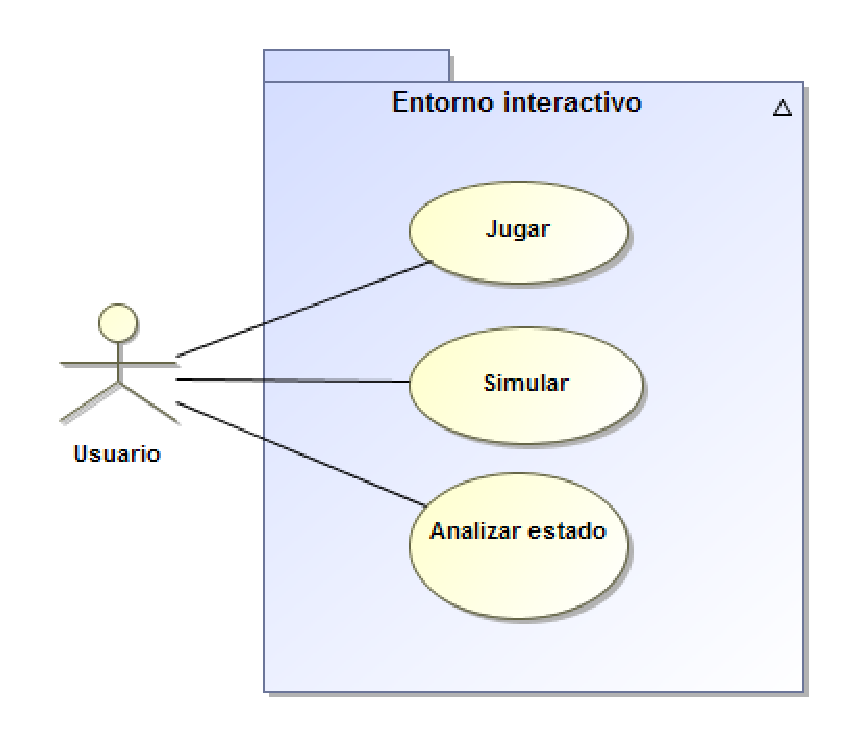
\includegraphics[scale=0.5]{contenido/cap5/imagenes/principales.eps}
	\caption{Diagrama de los principales casos de uso de la aplicación.}
	\label{fig:casos_uso_principales}
\end{figure}
\begin{enumerate}
	\item \begin{description}
		\item \textbf{Caso de uso:} Jugar\\
		El usuario juega una partida al juego elegido con los jugadores seleccionados. 
		\item \textbf{Extensión:} Si ninguno de los jugadores es humano, se muestra el desarrollo de la partida entre los jugadores controlados por el ordenador.
	\end{description}
	\item \begin{description}
		\item \textbf{Caso de uso:} Simular\\
		El usuario indica un número de partidas y la aplicación juega las partidas entre los dos jugadores seleccionados. El desarrollo de las partidas no se muestra. 
		\item \textbf{Precondición:} Ambos jugadores deben ser controlados por el ordenador, en caso contrario la opción de simular estará desactivada.
	\end{description}
	\item \begin{description}
		\item \textbf{Caso de uso:} Analizar estado\\
		El usuario crea un estado concreto del juego elegido, colocando manualmente las fichas sobre el tablero. A partir de ese estado, los jugadores seleccionados realizan independientemente un único movimiento cada uno.
		\item \textbf{Precondición:} Ambos jugadores deben ser controlados por el ordenador, en caso contrario la opción de analizar estado estará desactivada.
	\end{description}
\end{enumerate}
Cada uno de estos casos de uso produce unas estadísticas diferentes que son mostradas al finalizar los mismos.
Parte de esta información depende del jugador seleccionado; cada estrategia proporciona sus propias estadísticas, que son independientes del caso de uso elegido.
La aplicación permite además generar un informe en texto plano con toda la información de las estadísticas obtenidas.
Una vez terminado un caso de uso, los jugadores se pueden reutilizar para iniciar otro caso de uso sin tener en cuenta las estadísticas anteriores; lo que permite realizar tantas pruebas como se desee.

A continuación se presentan los casos de uso pertenecientes a la selección y configuración de los juegos y de las estrategias.
Para los juegos tenemos un único caso de uso (seleccionar juego) con la opción de modificar sus parámetros. La figura~\ref{fig:casos_uso_juegos} muestra el diagrama para este caso de uso.

\begin{figure}[b]
	\centering
	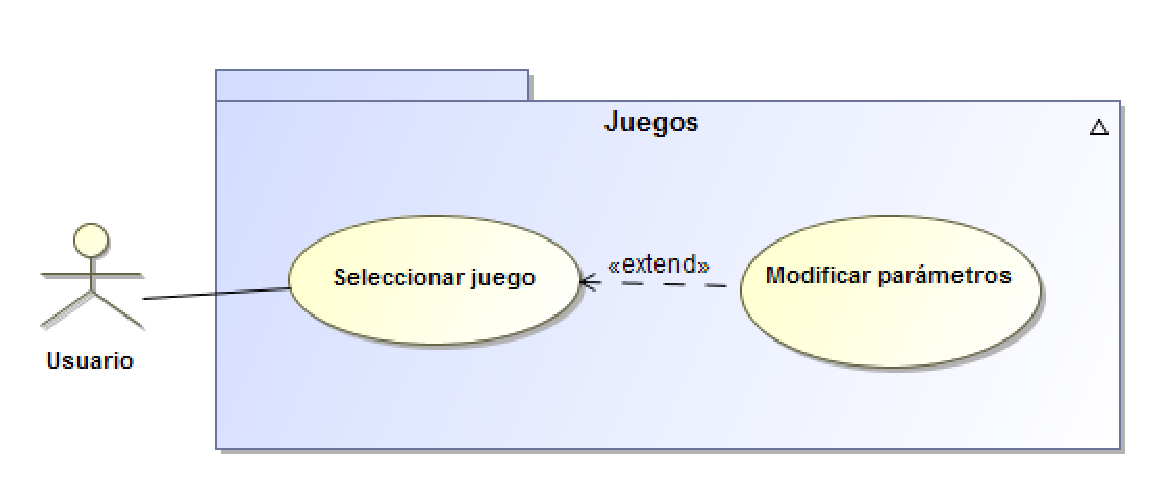
\includegraphics[scale=0.5]{contenido/cap5/imagenes/seleccionarJuego.eps}
	\caption{Diagrama de casos de uso para los juegos.}
	\label{fig:casos_uso_juegos}
\end{figure}

\begin{enumerate}[resume]
%\renewcommand{\labelitemi}{$\bullet$}
%\renewcommand{\labelitemii}{-}
	\item \begin{description}
		\item \textbf{Caso de uso:} Seleccionar juego \\
		El usuario elige el juego deseado de entre los disponibles.	
		\item \textbf{Extensión:} El usuario configura el juego seleccionado. Los parámetros a configurar dependen del juego:
		\begin{itemize}
	\item Conecta-4: El usuario elige el tamaño del tablero y la longitud ganadora de fichas.
	\item Go: El usuario elige el tamaño del tablero, las reglas de puntuación y los puntos de ventaja para el segundo jugador.
	\end{itemize}
	\end{description}
\end{enumerate}

En el caso de las estrategias, existen dos casos de uso: uno para seleccionar la estrategia del primer jugador y otro para seleccionar la estrategia del segundo jugador.
El escenario principal de ambos casos de uso es idéntico, por lo que sólo se describe uno de forma general. 
El diagrama de la figura~\ref{fig:casos_uso_estrategias} muestra el caso de uso de forma genérica para ambos jugadores.
\begin{figure}[h]
	\centering
	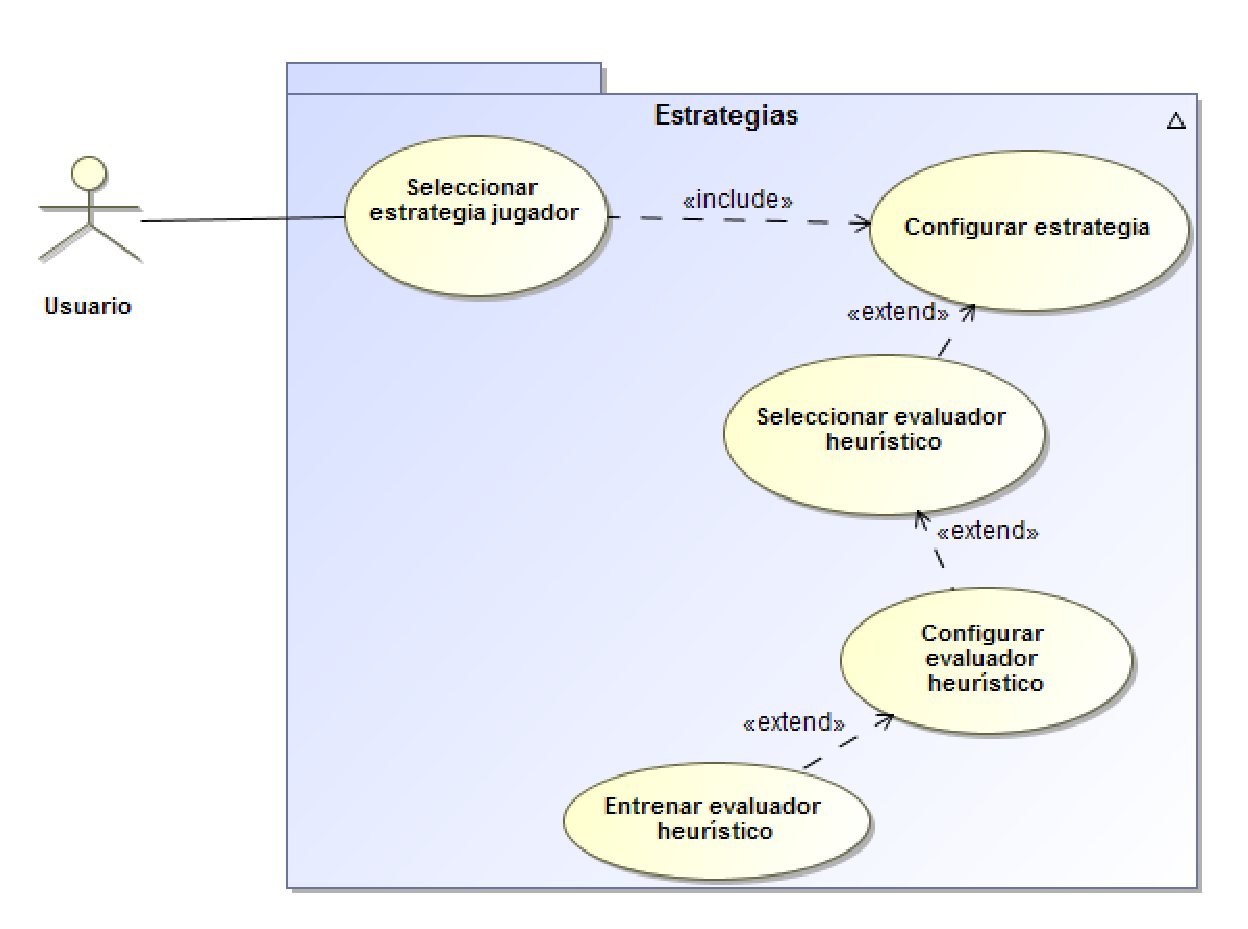
\includegraphics[scale=0.5]{contenido/cap5/imagenes/seleccionarEstrategia.eps}
	\caption{Diagrama de casos de uso para las estrategias.}
	\label{fig:casos_uso_estrategias}
\end{figure}
\begin{enumerate}[resume]
	\item \begin{description}
		\item \textbf{Caso de uso:} Seleccionar estrategia del jugador \\
		El usuario selecciona y configura los parámetros de la estrategia para uno de los jugadores.
		\item \textbf{Precondición:} El usuario ha seleccionado un juego.
		\item \textbf{Extensiones:}\\
		\begin{enumerate}
		 \renewcommand{\labelenumii}{\arabic{enumi}\alph{enumii}.}  
		 \renewcommand{\labelenumiii}{\arabic{enumi}\alph{enumii}.\arabic{enumiii}.}
		 \renewcommand{\labelenumiv}{\arabic{enumi}\alph{enumii}.\arabic{enumiii}\alph{enumiv}.}
			\item El usuario selecciona un evaluador heurístico.
			\begin{enumerate}
				\item El usuario configura el evaluador heurístico seleccionado.
				\begin{enumerate}
					\item El usuario configura el entrenamiento y la aplicación entrena el evaluador heurístico.
				\end{enumerate}				 
			\end{enumerate}
		\end{enumerate}
	\end{description}
\end{enumerate}
 